\documentclass[12pt, a4paper]{report}
\usepackage{graphicx, array, amsthm, amssymb, amsmath, algorithm, algpseudocode, float, xcolor, thmtools, thmbox, exercise, listings}
\usepackage[english]{babel}

\makeatletter
\renewcommand\thmbox@headstyle[2]{\bfseries #1}
\makeatother
\newtheorem[style=M,bodystyle=\normalfont]{theorem}{Theorem}
\newtheorem[style=M,bodystyle=\normalfont]{corollary}{Corollary}
\newtheorem[style=M,bodystyle=\normalfont]{lemma}{Lemma}
\newtheorem[style=M,bodystyle=\normalfont]{definition}{Definition}

\definecolor{dkgreen}{rgb}{0,0.6,0}
\definecolor{gray}{rgb}{0.5,0.5,0.5}
\definecolor{mauve}{rgb}{0.58,0,0.82}
\lstset{frame=tb,
  language=Java,
  aboveskip=3mm,
  belowskip=3mm,
  showstringspaces=false,
  columns=flexible,
  basicstyle={\small\ttfamily},
  numbers=none,
  numberstyle=\tiny\color{gray},
  keywordstyle=\color{blue},
  commentstyle=\color{dkgreen},
  stringstyle=\color{mauve},
  breaklines=true,
  breakatwhitespace=true,
  tabsize=3
}


\title{Foundation Of Operations Research \\ \textit{Exercises}}
\author{Christian Rossi}
\date{Academic Year 2023-2024}

\begin{document}

\maketitle

\newpage

\begin{abstract}
    Operations Research is the branch of applied mathematics dealing with quantitative methods to analyze and solve
    complex real-world decision-making problems. 
    
    The course covers some fundamental concepts and methods of Operations Research pertaining to graph optimization, 
    linear programming and integer linear programming. 
    
    The emphasis is on optimization models and efficient algorithms with a wide range of important applications in 
    engineering and management.  
\end{abstract}

\newpage

\tableofcontents

\newpage

\chapter{Exercise session I}
\begin{Exercise}[label=1]
    A bank has a capital of $C$ billions of Euro and two available stocks:
    \begin{enumerate}
        \item With an annual revenue of $15\%$ and risk factor of $\dfrac{1}{3}$. 
        \item With an annual revenue of $25\%$ and risk factor of $1$.
    \end{enumerate}
    The risk factor represents the maximum fraction of the stock value that can be lost. A risk factor of $25\%$ implies that, if stocks are bought for $100$ euro up to $25$ euro 
    can be lost. It is required that at least half of $C$ is risk-free. The amount of money used to buy stocks of two must not be larger than two times that used to buy stocks of one. 
    At least $\dfrac{1}{6}$ of C must be invested into one. 
    
    Give a Linear Programming formulation for the problem of determining an optimal portfolio for which the profit is maximized. 
    Solve the problem graphically.
\end{Exercise}
\begin{Answer}[ref=1]
    \begin{itemize}
        \item The parameters are: 
            \begin{itemize}
                \item The quantity of available capital $C$. 
            \end{itemize}
        \item The decision variables are:
            \begin{itemize}
                \item The amount of money invested in stock of type one $x_1$. 
                \item The amount of money invested in stock of type two $x_2$. 
            \end{itemize}
        \item The objective function is: 
            \[\max{\left[0.15x_1+0.25x_2\right]}\]
        \item The constraints are:
            \begin{itemize}
                \item Maximum capital: 
                    \[x_1+x_2 \leq C\]
                \item Half of the invested capital is risk-free:
                    \[\dfrac{1}{3}x_1+x_2 \leq \dfrac{C}{2}\]
                \item The amount of money used to buy stocks of two must not be larger than two times that used to buy stocks of one:
                    \[x_2 \leq 2x_1\]
                \item At least $\dfrac{1}{6}$ of $C$ must be invested into one: 
                    \[x_1 \geq \dfrac{1}{6}C\]
                \item Constraint on the variables:
                    \[x_1,x_2 \geq 0\]
            \end{itemize}
    \end{itemize}
    To solve the problem graphically, we must identify the feasible region in $\mathbb{R}^2$ that satisfies the constraints. To draw a constraint, it suffices to find any two points 
    that satisfy it with equality (as an equation). The border of the constraint is then represented by the only line containing such points. There are two possible ways to identify 
    which of the two half planes is the feasible one:
    \begin{itemize}
        \item In the first one, it suffices to pick a random point and checking whether it satisfies the constraint. If it does, the half space to which the point belongs is the
        feasible one, otherwise the other half space is.
        \item Alternatively, we can consider the gradient of the constraint and compare it to the direction of the inequality. 
    \end{itemize}
    The region found with the constraints is the following:
    \begin{figure}[H]
        \centering
        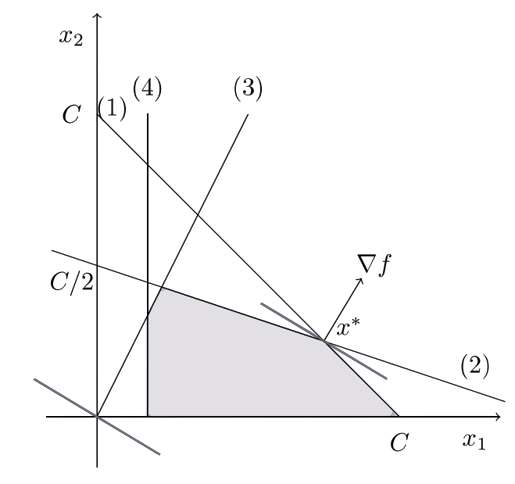
\includegraphics[width=0.5\linewidth]{images/plane.png}
    \end{figure}
    The feasible region is as shown in the picture. To find the feasible point where the objective function attains its maximal value, we can draw the level curves 
    $f(x_1,x_2)=0.15x_1+0.25x_2=z$ where each level curve is the set of points whose objective function value is equal to $z$, for any constant $z$. 
    
    Since $f$ is linear, the level curve $f(x_1,x_2) = z$ is a line, orthogonal to its gradient, and parametric in $z$. When $z$ is increased, we obtain parallel level lines that 
    move towards the direction of the gradient $\nabla f (x_1,x_2)$. 

    Note that, by starting with $z = 0$ and by increasing it in a continuous way, the level lines of f will first intersect the feasible region at $\left(\dfrac{C}{6}, 0\right)$, and then, 
    increasing $z$, at any other point, until the intersection is empty. The last feasible point having a nonempty intersection is the maximizer of $f$ over the feasible set. 
    In this problem there is a single maximizer. The maximizer, denoted by $x^{*}$, can be found as the solution to the following linear system: 
    \[
    \begin{cases}
        x_1+x_2 = C \\
        \dfrac{1}{3}x_1+x_2 = \dfrac{C}{2}
    \end{cases} 
    \]
    which yields $x^{*}=\left( \dfrac{3C}{4},\dfrac{C}{4} \right)$, where $f(x^{*})=\dfrac{7C}{40}$.
\end{Answer}

\newpage

\begin{Exercise}[label=2]
    A refinery produces two types of gasoline, mixing three basic oils according to the following gasoline mixture rules:
    \begin{table}[H]
        \centering
        \begin{tabular}{c|ccc|c|}
        \cline{2-5}
        \textbf{}                        & \textbf{Oil 1} & \textbf{Oil 2} & \textbf{Oil 3} & \textbf{Revenue} \\ \hline
        \multicolumn{1}{|c|}{Gasoline A} & $\leq 30\%$    & $\geq 40\%$    & -              & 5.5              \\
        \multicolumn{1}{|c|}{Gasoline B} & $\leq 40\%$    & $\geq 10\%$    & -              & 4.5              \\ \hline
        \end{tabular}
    \end{table}
    The last column of the previous table indicates the profit (euro/barrel). The availability of each type of oil (in barrel) and the cost (euro/barrel) are as follows:
    \begin{table}[H]
        \centering
        \begin{tabular}{c|c|c}
        \textbf{Oil} & \textbf{Availability} & \textbf{Cost} \\ \hline
        1            & 3 000                 & 3             \\
        2            & 2 000                 & 6             \\
        3            & 4 000                 & 4            
        \end{tabular}
    \end{table}
    Give a Linear Programming formulation for the problem of determining a mixture that maximizes the profit (difference between revenues and costs).
\end{Exercise}
\begin{Answer}[ref=2]
    \begin{itemize}
        \item The decision variables are:
            \begin{itemize}
                \item The amount of the $i$-th oil used to produce the $j$-th gasoline, $i \in \{1,2,3\}$ and $j \in \{A,B\}$ $x_{ij}$. 
                \item The amount of gasoline of type $j$-th that is produced, $j \in \{A,B\}$ $y_j$. 
            \end{itemize}
        \item The objective function is: 
            \[\max{5.5y_A+4.5y_B+3(x_{1A}+x_{1B})-6(x_{2A}+x_{2B})-4(x_{3A}+x_{3B})}\]
        \item The constraints are:
            \begin{itemize}
                \item Availability of 1: 
                    \[x_{1A}+x_{1B} \leq 3 000\]
                \item Availability of 2:
                    \[x_{2A}+x_{2B} \leq 2 000\]
                \item Availability of 3:  
                    \[x_{3A}+x_{3B} \leq 4 000\]
                \item Conservation of A:
                    \[y_A=x_{1A}+x_{2A}+x_{3A}\]
                \item Conservation of B:
                    \[y_B=x_{1B}+x_{2B}+x_{3B}\]
                \item Minimum quantity of $A$: 
                    \[x_{1A} \leq 0.3y_A\]
                \item Minimum quantity of $B$: 
                    \[x_{1B} \leq 0.5y_B\]
                \item Maximum quantity of $A$: 
                    \[x_{2A} \geq 0.4y_A\]
                \item Maximum quantity of $B$: 
                    \[x_{2B} \geq 0.1y_B\]
                \item The variable must be non-negative: 
                    \[x_{1A},x_{2A},x_{3A},x_{1B},x_{2B},x_{3B},y_A,y_B \geq 0\]  
            \end{itemize}
    \end{itemize}
\end{Answer}

\newpage

\newpage

\chapter{Exercise session II}
    \begin{Exercise}[label=3]
        Assume that $n$ packets of data must be routed from node $s$ to node $t$, along one of two available links, with capacity (bandwidth)$ k_1 = 1 \: Mbps$ and $k_2 = 2 \: Mbps$. 
        \begin{figure}[H]
            \centering
            
\includegraphics[width=0.3\linewidth]{images/link.png}
        \end{figure}
        The cost per unit of capacity of link $2$ is $30\%$ larger than that of link $1$. The following table indicates the quantity of capacity consumed by each packet 
        $i$, $i \in {l,\dots,n}$, and the cost to route it on link $1$. 
        \begin{table}[H]
            \centering
            \begin{tabular}{c|cc}
            \textbf{Packet} & \textbf{Consumed capacity} & \textbf{Cost on link one} \\ \hline
            1               & 0.3                        & 200                       \\
            2               & 0.2                        & 200                       \\
            3               & 0.4                        & 250                       \\
            4               & 0.1                        & 150                       \\
            5               & 0.2                        & 200                       \\
            6               & 0.2                        & 200                       \\
            7               & 0.5                        & 700                       \\
            8               & 0.1                        & 150                       \\
            9               & 0.1                        & 150                       \\
            10              & 0.6                        & 900                      
            \end{tabular}
        \end{table}
        Give an integer linear programming formulation for the problem of minimizing the total cost of routing all the packets. Give also an integer linear programming formulation for 
        the more general case where $m$ links are available. 
    \end{Exercise}
    \begin{Answer}[ref=3]
        The 2-link case can be formulated as the following integer linear program. 
        \begin{itemize}
            \item The sets are: 
                \begin{itemize}
                    \item The set of packets $I=\{1,\dots,n\}$. 
                    \item The set of links $J=\{1,\dots,m\}$. 
                \end{itemize}
            \item The parameters are: 
                \begin{itemize}
                    \item The capacity consumed by packet $i$, for $i \in I$ $a_i$.
                    \item The routing cost for packet $i$ on link $j$, for $i \in I,j \in J$ $c_{ij}$.
                    \item The capacity for link $j$ and $j \in J$ $k_{j}$. 
                \end{itemize}
            \item The decision variables are:
                \begin{itemize}
                    \item $x_ij$: $1$ if packet $i$ is routed on link $j$, or 0 otherwise, for $i \in I,j \in J$
                \end{itemize}
            \item The objective function is: 
                \[\min{\sum_{i \in I}{c_{ij}x_{ij}}}\]
            \item The constraints are:
                \begin{itemize}
                    \item The assignment: 
                        \[\sum_{j \in J}x_{ij} = 1\]
                    \item The capacity: 
                        \[\sum_{j \in J}a_ix_{ij} \leq k_j\]
                    \item The variables must be binary: 
                        \[x_{ij} \in \{0,1\} \:\:\:\:\:\: i \in I,j \in J\]
                \end{itemize}
        \end{itemize}
        The $m$-link formulation requires a new set of binary variables, one for each packet and link. The packet-to-link assignment is also to be explicitly introduced. 
    \end{Answer}

    \newpage 

    \begin{Exercise}[label=4]
        A company $A$, which produces one type of high-precision measuring instrument, has to plan the production for the next 3 months. Each month, $A$ can produce at most 110 units, 
        at a unit cost of 300 Euro. Moreover, each month, up to 60 additional units produced by another company B can be bought at a unit cost of 330 Euro. Unsold units can be 
        stored. The inventory cost is of 10 Euro per unit of product, per month. Sales forecasts indicate a demand of 100, 130, and 150 units of product for the next 3 months.
        \begin{enumerate}
            \item Give a linear programming formulation for the problem of determining a production plan (direct or indirect) which minimizes the total costs, while satisfying 
                the monthly demands.
            \item Give a mixed integer linear programming formulation for the variant of the problem where production lots have a minimum size. In particular, if any strictly 
                positive quantity is produced in a given month, this quantity cannot be smaller than 15 units. 
        \end{enumerate}
    \end{Exercise}
    \begin{Answer}[ref=4]
        \begin{enumerate}
            \item \begin{itemize}
                    \item The sets are: 
                        \begin{itemize}
                            \item The set of months $T=\{1,2,3\}$. 
                        \end{itemize}
                    \item The parameters are: 
                        \begin{itemize}
                            \item The production capacity of $A$ $b$. 
                            \item The production capacity of $B$ $b^{'}$. 
                            \item The unit production cost for $A$ $c$. 
                            \item The unit production cost for $B$ $c^{'}$. 
                            \item The inventory cost per unit and month $m$. 
                            \item The sales forecast for month $t$, for $t \in T$ $d_t$. 
                        \end{itemize}
                    \item The decision variables are:
                        \begin{itemize}
                            \item The units produced by $A$ in month $t$, $t \in T$ $x_t$. 
                            \item The units bought from $B$ in month $t$, for $t \in T$ $x_t$ $x_t^{'}$.
                            \item The units in inventory at the end of month $t$, for $t \in T \cup \{0\}$ $z_t$. 
                        \end{itemize}
                    \item The objective function is: 
                        \[\min{\sum_{t \in T}{cx_t+c^{'}x_t^{'}+mz_t}}\]
                    \item The constraints are:
                        \begin{itemize}
                            \item The capacity of $A$: 
                                \[x_t \leq b\]
                            \item The capacity of $A$: 
                                \[x_t^{'} \leq b^{'}\]
                            \item The demand: 
                                \[x_{t-1}+x_t+x_t^{'} \geq d_t\]
                            \item The inventory balance: 
                                \[x_{t-1}+x_t+x_t^{'}-d_t = z_tt\]
                            \item The starting condition: 
                                \[z_0=0\]
                            \item The non-negative variables: 
                                \[x_t,x_t^{'},z_t \geq 0\]
                            \end{itemize}
                \end{itemize}
            \item To take into account the minimum lot size, we add the binary variables $y_t$, that is $1$ if production is active at month $t$, or $0$ otherwise, for 
                $t \in T$ and the constraints: 
                \begin{itemize}
                    \item The minimum lot size: 
                        \[x_t \geq l_{y_t}\]
                    \item The activation: 
                        \[x_t \leq M_{y_t}\]
                \end{itemize}
                where $l = 15$ is the minimum lot size, and $M$ is a large enough value, such that constraint $x_t \leq M_{y_t}$ is redundant when $y_t=1$. For instance, 
                we can choose $M = 110$. Such constraints are usually called big-$M$ constraints. 
        \end{enumerate}
        
    \end{Answer}









\newpage

\chapter{Laboratory session I}
\begin{Exercise}[label=a]
    A canteen has to plan the composition of the meals that it provides. A meal can be composed of the types of food indicated in the following table. 
    Costs, in Euro per hg, and availabilities, in hg, are also indicated.
    \begin{table}[H]
        \centering
        \begin{tabular}{|c|c|c|}
        \hline
        \textbf{Food} & \textbf{Cost} & \textbf{Availability} \\ \hline
        Bread         & 0.1           & 4                     \\
        Milk          & 0.5           & 3                     \\
        Eggs          & 0.12          & 1                     \\
        Meat          & 0.9           & 2                     \\
        Cake          & 1.3           & 2                     \\ \hline
        \end{tabular}
    \end{table}
    A meal must contain at least the following amount of each nutrient: 
    \begin{table}[H]
        \centering
        \begin{tabular}{|c|c|}
        \hline
        Nutrient & Minimal quantity \\ \hline
        Calories & 600 cal          \\
        Proteins & 50 g             \\
        Calcium  & 0.7 g            \\ \hline
        \end{tabular}
    \end{table}
    Each hg of each type of food contains to following amount of nutrients: 
    \begin{table}[H]
        \centering
        \begin{tabular}{|cccc|}
        \hline
        \textbf{Food}               & \textbf{Calories}            & \textbf{Proteins}         & \textbf{Calcium} \\ \hline
        \multicolumn{1}{|c|}{Bread} & \multicolumn{1}{c|}{30 cal}  & \multicolumn{1}{c|}{15 g} & 0.02 g           \\
        \multicolumn{1}{|c|}{Milk}  & \multicolumn{1}{c|}{50 cal}  & \multicolumn{1}{c|}{15 g} & 0.15 g           \\
        \multicolumn{1}{|c|}{Eggs}  & \multicolumn{1}{c|}{150 cal} & \multicolumn{1}{c|}{30 g} & 0.05 g           \\
        \multicolumn{1}{|c|}{Meat}  & \multicolumn{1}{c|}{180 cal} & \multicolumn{1}{c|}{90 g} & 0.08 g           \\
        \multicolumn{1}{|c|}{Cake}  & \multicolumn{1}{c|}{400 cal} & \multicolumn{1}{c|}{70 g} & 0.01 g           \\ \hline
        \end{tabular}
    \end{table}
    Give a linear programming formulation for the problem of finding a meal of minimum total cost which satisfies the minimum nutrient requirements.
\end{Exercise}
\begin{Answer}[ref=a]
    \begin{lstlisting}[language=Python]
# Import the package mip
!pip install mip
import mip
# Food
I = {'Bread', 'Milk', 'Eggs', 'Meat', 'Cake'}
# Nutrients
J = {'Calories', 'Proteins', 'Calcium'}
# Cost in Euro per hg of food
c = {'Bread':0.1, 'Milk':0.5, 'Eggs':0.12, 'Meat':0.9, 'Cake':1.3}
# Availability per hg of food
q = {'Bread':4, 'Milk':3, 'Eggs':1, 'Meat':2, 'Cake':2}
# minum nutrients 
b = {'Calories':600, 'Proteins':50, 'Calcium':0.7}
# Nutrients per hf of food
a = {   ('Bread','Calories'):30,
        ('Milk','Calories'):50,
        ('Eggs','Calories'):150,
        ('Meat','Calories'):180,
        ('Cake','Calories'):400,
        ('Bread','Proteins'):5,
        ('Milk','Proteins'):15,
        ('Eggs','Proteins'):30,
        ('Meat','Proteins'):90,
        ('Cake','Proteins'):70,
        ('Bread','Calcium'):0.02,
        ('Milk','Calcium'):0.15,
        ('Eggs','Calcium'):0.05,
        ('Meat','Calcium'):0.08,
        ('Cake','Calcium'):0.01}
# Define a empty model
model = mip.Model()
# Define variables
x = [model.add_var(name = i,lb=0) for i in I]
# Define the objective function
model.objective = mip.minimize(mip.xsum())
# Availability constraint
for i,food in enumerate(I):
  model.add_constr()
# Minum nutrients constraint
for j in J:
  model.add_constr(mip.xsum()>=)
# Optimizing command
model.optimize()
# Optimal objective function value
model.objective.x
# Printing the variables values
for i in model.vars:
  print(i.name)
  print(i.x)
    \end{lstlisting}
\end{Answer}

\newpage

\end{document}